\section{Coxeter groups}
\label{sec:coxeter-groups}

A Coxeter group, named after Harold Scott MacDonald Coxeter, is an abstract group generated by involutions with specific relations between these generators. A simple class of a Coxeter groups are the symmetry groups of regular polyhedras in the Euclidean space.

The symmetry group of the square for example can be generated by two reflections $s,t$, whose stabilized hyperplanes enclose an angle of $\pi / 4$. In this case the map $st$ is a rotation in the plane by $\pi / 2$. So we have $s^2 = t^2 = (st)^4 = \id$. In fact this reflection group is determined up to isomorphy by $s,t$ and these three relations \cite[Theorem 1.9]{humphreys:coxeter}. Furthermore it turns out, that the finite reflection groups in the Euclidean space are precisely the finite Coxeter groups \cite[Theorem 6.4]{humphreys:coxeter}.

In this chapter we will compile some basic facts on Coxeter groups, based on \cite{humphreys:coxeter}.

%!TEX root = ../../../_main.tex
\subsection{Introduction to Coxeter groups}
\label{sec:coxeter-groups-introduction}

\begin{defi}
	\typedlabel{defi:coxeter-system}
	Let $S = \{ s_1, \ldots, s_n \}$ be a finite set of symbols and
	$$R = \{ m_{ij} \in \nn \cup \infty : 1 \leq i,j \leq n \}$$
	a set numbers (or $\infty$) with $m_{ii} = 1$, $m_{ij} > 1$ for $i \neq j$ and $m_{ij} = m_{ji}$. Then the free represented group
	$$W = \langle S \ | \ (s_i s_j)^{m_{ij}} \rangle$$
	is called a \defword{Coxeter group} and $(W,S)$ the corrosponding \defword{Coxeter system}. The cardinality of $S$ is called the \defword{rank} of the Coxeter system (and the Coxeter group).
\end{defi}

From the definiton we see, that Coxeter groups only depend on the cardinality of $S$ and the relations between the generators in $S$. A common way to visualize this information are Coxeter graphs.

\begin{defi}
	\typedlabel{defi:coxeter-graph}
	Let $(W,S)$ be a Coxeter system. Create a graph by adding a vertex for each generator in $S$. Let $(s_i s_j)^m = 1$. In case $m = 2$ the two corrosponding vertices have no connecting edge. In case $m = 3$ they are connected by an unlabed edge. For $m > 3$ they have an connecting edge with label $m$. This graph we call the \defword{Coxeter graph} of our Coxeter system $(W,S)$.
\end{defi}

\begin{defi}
	For an arbitrary element $w \in W$, $(W,S)$ a Coxeter system, we call a product $s_{i_1} \cdots s_{i_n} = w$ of generators $s_{i_1} \ldots s_{i_n} \in S$ an \defword{expression} of $w$. Any expression that can be obtained from $s_{i_1} \cdots s_{i_n}$ by omitting some (or all) factors is called a \defword{subexpression} of $w$.
\end{defi}

The present relations between the generators of a Coxeter group allow us to rewrite expressions. Hence an element $w \in W$ can have more than one expression. Obviously any element $w \in W$ has infinitly many expressions, since any expression $s_{i_1} \cdots s_{i_n} = w$ can be extended by applying $s_1^2 = 1$ from the right. But there must be a smallest number of generators needed to receive $w$. For example the neutral element $e$ can be expressed by the empty expression. Or each generator $s_i \in S$ can be expressed by itself, but any expression with less factors (i.e. the empty expression) is unequal to $s_i$.

\begin{defi}
	\typedlabel{defi:length-function}
	Let $(W,S)$ be a Coxeter system and $w \in W$ an element. Then there are some (not neseccarily distince) generators $s_i \in S$ with $s_1 \cdots s_r = w$. We call $r$ the \defword{expression length}. The smallest number $r \in \nn_0$ for that $w$ has an expression of length $r$ is called the \defword{length} of $w$ and each expression of $w$, that is ob minimal length, is called \defword{reduced expression}. The map
	$$ l : W \to \nn_0 $$
	that maps each element in $W$ to its length is called \defword{length function}.
\end{defi}

\begin{defi}
	Let $(W,S)$ be a Coxeter system. We define
	$$ D_R(w) := \{ s \in S : l(ws) < l(w) \} $$
	as the \defword{right descending set} of $w$. The analogue left version
	$$ D_L(w) := \{ s \in S : l(sw) < l(w) \} $$
	is called \defword{left descending set} of $w$. The right descending set will also just be called \defword{descending set} of $w$.
\end{defi}

The next lemma yields some useful identities and relations for the length function.

\begin{lemm}
	%\cite[Section 5.2]{humphreys:coxeter}
	\typedlabel{lemm:length-function-properties}
	Let $(W,S)$ be a Coxeter system, $s \in S$, $u, w \in W$ and $l : W \to \nn$ the length function. Then
	\begin{enumerate}
		\item $l(w) = l(w^{-1})$,
		\item $l(w) = 0$ iff $w = e$,
		\item $l(w) = 1$ iff $w \in S$,
		\item $l(uw) \leq l(u) + l(w)$,
		\item $l(uw) \geq l(u) - l(w)$ and
		\item $l(ws) = l(w) \pm 1$.
	\end{enumerate}

	\begin{proof}
		See \cite[Section 5.2]{humphreys:coxeter}.
	\end{proof}
\end{lemm}
%!TEX root = ../../../_main.tex
\subsection{Bruhat ordering}
\label{sec:coxeter-groups-bruhat-ordering}

We now investigate ways to partially order the elements of a Coxeter group. Futhermore, this ordering should be compatible with the length function. The most useful way to achieve this is the Bruhat ordering \cite[Section 5.9]{humphreys:coxeter}.

\begin{defi}
	\typedlabel{defi:poset}
	Let $M$ be a set. A binary relation, in this case often denoted as ``$\leq$'', is called a \defword{partial order} over $M$, if fullfills the following conditions for all $a,b,c \in M$:
	\begin{enumerate}
		\item $a \leq a$, called \defword{reflexivity}
		\item if $a \leq b$ and $b \leq a$ then $a=b$, called \defword{antisymmetry}
		\item if $a \leq b$ and $b \leq c$ then $a \leq c$, called \defword{transitivity}
	\end{enumerate}
	In this case $(M,\leq)$ is called a \defword{poset}. If two elements $a \leq b \in M$ are immediate neighbours, i.e. there is no third element $c \in M$ with $a \leq c \leq b$ we say that $b$ \defword{covers} $a$. A poset is called \defword{graded poset} if there is a map $\rho : M \to \nn$ so that $\rho(b) - 1 = \rho(a)$ whenever $b$ covers $a$. In this case $\rho$ is called the \defword{rank function} of the graded poset.
\end{defi}

\begin{defi}
	\typedlabel{defi:hasse-diagram}
	Let $(M,\leq)$ be a poset. The \defword{Hasse diagram} of the poset is the graph obtained in the following way: Add a vertex for each element in $M$. Then add a directed edge from vertex $a$ to $b$ whenever $b$ covers $a$.
\end{defi}

\begin{exam}
	Suppose we have an arbitrary set $M$. Then the powerset $\mathcal P (M)$ can be partially ordered by the subset relation, so $(\mathcal P (M), \subseteq)$ is a poset. Indeed this poset is always graded with the cardinality function as rank function. In Figure \ref{fig:poset-xyz-subsets} we see the Hasse diagram of this poset with $M = \{x,y,z\}$.

	\begin{figure}[ht]
		\centering
		%!TEX root = ../../_main.tex
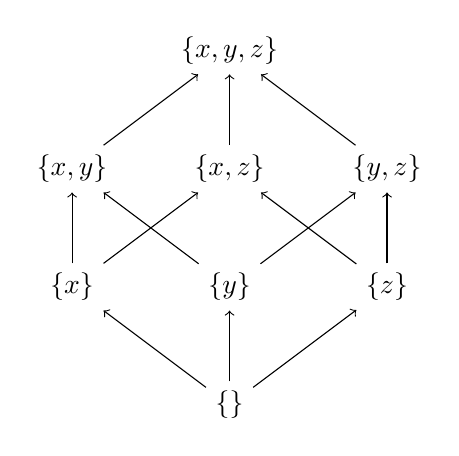
\begin{tikzpicture}
	\tikzstyle{every node}=[]
	\tikzstyle{relation}=[->]

	\node (xyz) at (0,0) {$\{x,y,z\}$};
	\node (xy) at (-2,-1.5) {$\{x,y\}$};
	\node (xz) at (0,-1.5) {$\{x,z\}$};
	\node (yz) at (2,-1.5) {$\{y,z\}$};
	\node (x) at (-2,-3) {$\{x\}$};
	\node (y) at (0,-3) {$\{y\}$};
	\node (z) at (2,-3) {$\{z\}$};
	\node (0) at (0,-4.5) {$\{\}$};
	\draw[relation] (0) -- (x);
	\draw[relation] (0) -- (y);
	\draw[relation] (0) -- (z);
	\draw[relation] (x) -- (xy);
	\draw[relation] (x) -- (xz);
	\draw[relation] (y) -- (xy);
	\draw[relation] (y) -- (yz);
	\draw[relation] (z) -- (xz);
	\draw[relation] (z) -- (yz);
	\draw[relation] (xy) -- (xyz);
	\draw[relation] (xz) -- (xyz);
	\draw[relation] (yz) -- (xyz);
\end{tikzpicture}
		\caption{Hasse diagram of the set of all subsets of $\{x,y,z\}$ order by the subset relation}
		\label{fig:poset-xyz-subsets}
	\end{figure}
\end{exam}

\begin{defi}
	\typedlabel{defi:bruhat-ordering}
	Let $(W,S)$ be a Coxeter system and $T = \cup_{w \in W} wSw^{-1}$ the set of all reflections in $W$. We write $w' \to w$ if there is a $t \in T$ with $w't = w$ and $l(w') < l(w)$. If there is a sequence $w' = w_0 \to w_1 \to \ldots \to w_m = w$ we say $w' < w$. The resulting relation $w' \leq w$ is called \defword{Bruhat ordering}, denoted as $\Br(W)$.
\end{defi}

\begin{lemm}
	\typedlabel{lemm:bruhat-ordering-is-poset}
	Let $(W,S)$ be a Coxeter system. Then $\Br(W)$ is a poset.

	\begin{proof}
		The Bruhat ordering is reflexive by definition. Since the elements in sequences $e \to w_1 \to w_2 \to \ldots$ are strictly ascending in length, it must be antisymmetric. By concatenation of sequences we get the transitivity.
	\end{proof}
\end{lemm}

What we really want is the Bruhat ordering to be graded with the length function as rank function. By definition we already have $v < w$ iff $l(v) < l(w)$, but its not that obvious that two immediately adjacent elements differ in length by exactly 1. Beforehand let us just mention two other partial orderings, where this property is obvious by definition:

\begin{defi}
	Let $(W,S)$ be a Coxeter system. The ordering $\leq_R$ defined by $u \leq_R w$ iff $uv = w$ for some $u \in W$ with $l(u) + l(v) = l(w)$ is called the \defword{right weak ordering}. The left sided version $u \leq_L w$ iff $vu = w$ is called the \defword{left weak ordering}.
\end{defi}

To ensure the Bruhat ordering is graded as well, we need another characterization of the Bruhat ordering with subexpressions. As we show it is $u \leq w$ iff there is a reduced expression of $u$ that is a subexpression of a reduced expression of $w$.

\begin{prop}
	%\cite[Prop 5.9]{humphreys:coxeter}
	\typedlabel{prop:u-leq-w-then-us-leq-w-or-us-leq-ws}
	Let $(W,S)$ be a Coxeter system, $u,w \in W$ with $u \leq w$ and $s \in S$. Then $us \leq w$ or $us \leq ws$ or both.

	\begin{proof}
		We can reduce the proof (\todo why?) to the case $u \to w$, i.e. $ut = w$ for a $t \in T$ with $l(v) < l(u)$. Let $s = t$. Then $us \leq w$ and we are done. In case $s \neq t$ there are two alternatives for the lengths. We can have $l(us) = l(u) - 1$ which would mean $us \to u \to w$, so $us \leq w$.

		Assume $l(us) = l(u) + 1$. For the reflection $t' = sts$ we get $(us)t' = ussts = uts = ws$. So it is $us \leq ws$ iff $l(us) < l(ws)$. Suppose this is not the case. Since we have assumed $l(us) = l(u) + 1$ any reduced expression $u = s_1 \cdots s_r$ for $u$ yields a reduced expression $us = s_1 \cdots s_r s$ for $us$. With the \ref{theo:strong-exchange-condition} we can obtain $ws = ust'$ from $us$ by omitting one factor. This omitted factor cannot be $s$ since $s \neq t$. This means $ws = s_1 \cdots \hat s_i \cdots s_r s$ and so $ws = s_1 \cdots \hat s_i \cdots s_r$, contradicting to our assumption $l(u) < l(w)$
	\end{proof}
\end{prop}

\begin{theo}
	%\cite[Theorem 5.10]{humphreys:coxeter}
	\typedlabel{theo:bruhat-subexpression-characterization}
	Let $(W,S)$ be a Coxeter system and $w \in W$ with any reduced expression $w = s_1 \cdots s_r$ and $s_i \in S$. Then $u \leq w$ (in the Bruhat ordering) iff $u$ can be obtained as a subexpression of this reduced expression.

	\begin{proof}
		\todo
	\end{proof}
\end{theo}

This characterization of the Bruhat ordering is very handy. With it and the following short lemma we will be in the position to show, that $\Br(W)$ is graded with rank function $l$.

\begin{lemm}
	%\cite[Lemma 5.11]{humphreys:coxeter}
	\typedlabel{lemm:dont-know}
	Let $(W,S)$ be a Coxeter system, $u,w \in W$ with $u < w$ and $l(w) = l(u) + 1$. In case there is a generator $s \in S$ with $u < us$ but $us \neq w$, then both $w < ws$ and $us < ws$.

	\begin{proof}
		Due to \ref{prop:u-leq-w-then-us-leq-w-or-us-leq-ws} we have $us \leq w$ or $us \leq ws$. Since $l(us) = l(w)$ and $us \neq w$ the first case is impossible. So $us \leq ws$ and because of $u \neq w$ already $us < ws$. In turn, $l(w) = l(us) < l(ws)$, forcing $w < ws$.
	\end{proof}
\end{lemm}

\begin{prop}
	%\cite[Proposition 5.11]{humphreys:coxeter}
	\typedlabel{prop:bruhat-intervals}
	Let $(W,S)$ be a Coxeter system and $u < w$. Then there are elements $w_0,\ldots,w_m \in W$ such that $u = w_0 < w_1 < \ldots < w_m = w$ with $l(w_i) = l(w_{i-1}) + 1$ for $1 \leq i \leq m$.

	\begin{proof}
		We induce on $r = l(u) + l(w)$. In case $r = 1$ we have $u = e$ and $w = s$ for an $s \in S$ and are done. Conversely suppose $r > 1$. Then there is a reduced expression $w = s_1 \cdots s_r$ for $w$. Lets fix this expression. Then $l(w s_r) < l(w)$. Thanks to \ref{theo:bruhat-subexpression-characterization} there must be a subexpression of $w$ with $u = s_{i_1} \cdots s_{i_q}$ for some $i_1 < \ldots < i_q$. We distinguish between two cases:

		\begin{description}
			\item[$u < us$] If $i_q = r$, then $us = s_{i_1} \cdots s_{i_q} s = s_{i_1} \cdots s_{i_{q-1}}$ which is also a subexpression of $ws$. This yields $u < us \leq ws < w$. Since $l(ws) < r$ there is, by induction, a sequence of the desired form. The last step from $ws$ to $w$ also differs in length by exactly 1, so we are done. If $i_q < r$ then $u$ is itself already a subexpression of $ws$ and we can again find a sequence from $u$ to $ws$ strictly ascending length by 1 in each step and have one last step from $ws$ to $w$ also increasing length by 1.
			\item[$us < u$] Then by induction we can find a sequence from $us$ to $w$, say $us = w_0 < \ldots < w_m = w$, where the lengths of neighboured elements differ by exactly 1. Since $w_0 s = u > us = w_0$ and $w_m s = ws < w = w_m$ there must be a smallest index $i \geq 1$, such that $w_i s < w_i$, which we choose. Suppose $w_i \neq w_{i-1} s$. It is $w_{i-1} < w_{i-1}s \neq w_i$ and due to \ref{lemm:dont-know} we get $w_i < w_i s$. This contradicts to the minimality of $i$. So $w_i = w_{i-1} s$. For all $1 \leq j < i$ we have $w_j \neq w_{j-1} s$, because of $w_j < w_j s$. Again we apply \ref{lemm:dont-know} to receive $w_{j-1} s < w_j s$. Alltogether we can construct a sequence
			$$ u = w_0 s < w_1 s < \ldots < w_{i-1} s = w_i < w_{i+1} < \ldots w_m = w, $$
			which matches our assumption. \qedhere
		\end{description}
	\end{proof}
\end{prop}

\begin{coro}
	\typedlabel{coro:bruhat-ordering-is-graded}
	Let $(W,S)$ be a Coxeter system and $\Br(W)$ the Bruhat ordering poset of $W$. Then $\Br(W)$ is graded with $l:W \to \nn$ as rank function.

	\begin{proof}
		Let $u,w \in W$ with $w$ covering $u$. Then \ref{prop:bruhat-intervals} says there is a sequence $u = w_0 < \ldots < w_m = w$ with $l(w_i) = l(w_{i-1}) + 1$ for $1 \leq i \leq m$. Since $w$ covers $u$ it must be $m = 1$ and so $u < w$ with $l(w) = l(u) + 1$.
	\end{proof}
\end{coro}

\begin{theo}[Lifting Property]
	%\cite[Theorem 1.1]{deodhar:bruhat-order}
	\namedlabel{theo:lifting-property}
	Let $(W,S)$ be a Coxeter system and $v,w \in W$ with $v \leq w$. Suppose $s \in S$ with $s \in D_R(w)$. Then
	\begin{enumerate}
		\item $vs \leq w$,
		\item $s \in D_R(v) \Rightarrow vs \leq ws$.
	\end{enumerate}

	\begin{proof}
		We use the alternative subexpression characterization of the Bruhat ordering from \ref{theo:bruhat-subexpression-characterization}.
		\begin{enumerate}
			\item Since $s \in D_R(w)$ there exists a reduced expression $w = s_1 \cdots s_r$ with $s_r = s$. Due to $v \leq w$ we can obtain $v$ as a subexpression $v = s_{i_1} \cdots s_{i_q}$ from $w$. If $i_q = r$ then $vs = s_{i_1} \cdots s_{i_q} s = s_{i_1} \cdots s_{i_{q - 1}}$ is also a subexpression of $w$. Else, if $i_q \neq r$ then $v$ is a subexpression of $ws = s_1 \cdots s_{r-1}$ and so $vs$ is again a subexpression of $w = s_1 \cdots s_{r-1} s$. In both cases we get $vs \leq w$.
			\item If we additionally assume $s \in D_R(v)$ then we can always find a reduced expression $w = s_1 \cdots s_r$ with $s_r = s$ having $u = s_{i_1} \cdots s_{i_q}$ as subexpression with $s_{i_q} = s$. This yields $vs = s_{i_1} \cdots s_{i_{q-1}} \leq s_1 \cdots s_{r-1} = ws$. \qedhere
		\end{enumerate}
	\end{proof}
\end{theo}

The \ref{theo:lifting-property} seems quite innocent, but when trying to investigate facts around the Bruhat ordering it proofs to be one of the key tools in many cases.
%!TEX root = ../../../_main.tex
\subsection{Exchange and Deletion Condition}
\label{sec:coxeter-groups-exchange-deletion-condition}

We now obtain a way to get a reduced expression of an arbitrary element $s_1 \cdots s_r = w \in W$.

\begin{defi}
	\typedlabel{defi:reflection}
	Let $(W,S)$ be a Coxeter system. Any element $w \in W$ that is conjugated to an generator $s \in S$ is called \defword{reflection}. Hence the set of all reflections in $W$ is
	$$ T = \bigcup_{w \in W} wSw^{-1}. $$
\end{defi}

\begin{theo}[Strong Exchange Condition]
	\namedlabel{theo:strong-exchange-condition}
	\theocite{Theorem 5.8}{humphreys:coxeter}
	Let $(W,S)$ be a Coxeter system, $w \in W$ an arbitrary element and ${s_1 \cdots s_r = w}$ with $s_i \in S$ a not necessarily reduced expression for $w$. For each reflection $t \in T$ with $l(wt) < l(w)$ there exists an index $i$ for which $wt = s_1 \cdots \hat s_i \cdots s_r$, where $\hat s_i$ means omission. In case we start from a reduced expression, then $i$ is unique.
\end{theo}

The \ref{theo:strong-exchange-condition} can be weaken, when insisting on $t \in S$ to receive the following corollary.

\begin{coro}[Exchange Condition]
	\namedlabel{coro:exchange-condition}
	Let $(W,S)$ be a Coxeter system, $w \in W$ an arbitrary element and ${s_1 \cdots s_r = w}$ with $s_i \in S$ a not necessarily reduced expression for $w$. For each generator $s \in S$ with $l(ws) < l(w)$ there exists an index $i$ for which $ws = s_1 \cdots \hat s_i \cdots s_r$, where $\hat s_i$ means omission. In case we start from a reduced expression, then $i$ is unique.

	\begin{proof}
		Directly from \ref{theo:strong-exchange-condition}.
	\end{proof}
\end{coro}

\begin{rema}
	\typedlabel{rema:exchange-condition-left-sided}
	Note that both, \ref{theo:strong-exchange-condition} and \ref{coro:exchange-condition} have an analogues left-sided version
	$$ l(tw) < l(w) \Rightarrow tw = t s_1 \cdots s_k = s_1 \cdots \hat s_i \cdots s_k $$
	for all reflections $t \in T$, hence for all generators $s \in S$ in particular.
\end{rema}

\begin{coro}[Deletion Condition]
	\namedlabel{coro:deletion-condition}
	\theocite{Corollary 5.8}{humphreys:coxeter}
	Let $(W,S)$ be a Coxeter system, $w \in W$ and $w = s_1 \cdots s_r$ with $s_i \in S$ an unreduced expression of $w$. Then there exist two indices $i,j \in \{1,\cdots,r\}$ with $i < j$, such that $w = s_1 \cdots \hat s_i \cdots \hat s_j \cdots s_r$, where $\hat s_i$ and $\hat s_j$ mean omission.

	\begin{proof}
		Since the expression is unreduced there must be an index $j$ for that the twisted length shrinks. That means for $w' = s_1 \cdots s_{j-1}$ is $l(w' s_j) < l(w')$. Using the \ref{coro:exchange-condition} we get $w' s_j = s_1 \cdots \hat s_i \cdots s_{j-1}$ yielding $w = s_1 \cdots \hat s_i \cdots \hat s_j \cdots s_r$.
	\end{proof}
\end{coro}

This corollary is called \defword{Deletion Condition} and allows us to reduce expressions, i.e. to find a subexpression that is reduced. Due to the Deletion Condition any unreduced expression can be reduced by omitting an even number of generators (we just have to apply the Deletion Condition inductively).

The \ref{theo:strong-exchange-condition}, the \ref{coro:exchange-condition} and the \ref{coro:deletion-condition}, are some of the most powerful tools when investigating properties of Coxeter groups. We can use the second to prove a very handy property of Coxeter groups. The intersection of two parabolic subgroups is again a parabolic subgroup.

\begin{defi}
	\typedlabel{defi:parabolic-subgroup}
	Let $(W,S)$ be a Coxeter system. For a subset of generators $I \subset S$ we call the subgroup $W_I \leq W$, that is generated by the elements in $I$ with the corrosponding relations, a \defword{parabolic subgroup} of $W$.
\end{defi}

\begin{lemm}
	\typedlabel{lemm:w-reduced-expression-letters-independent}
	\theocite{Section 5.8}{humphreys:coxeter}
	Let $(W,S)$ be a Coxeter system and $w \in W$. Let $w = s_1 \cdots s_k$ any reduced expression for $w$. Then $\{s_1, \ldots, s_k\} \subset S$ is independent of the particular choosen reduced expression. It only depends on $w$ itself.
\end{lemm}

This means, that two reduced expressions for an element $w \in W$ use exactly the same generators. A related fact, is the following lemma.

\begin{lemm}
	\theocite{Section 5.8}{humphreys:coxeter}
	Let $(W,S)$ be a Coxeter system and $I,J \subset S$ two subsets of generators. Then ${W_I \cap W_J} = W_{I \cap J}$.
\end{lemm}
\subsection{Finite Coxeter groups}

Coxeter groups can be finite and infinite. A simple example for the former category is the following. Let $S = \{ s \}$. Due to definition it must be $s^2 = e$. So $W$ is isomorph to $\zz_2$ and finite. An example for an infinite Coxeter group can be obtained from $S = \{s,t\}$ with $s^2=t^2=e$ and $(st)^\infty = e$ (so we have no relation between $s$ and $t$). Obviously the element $st$ has infinite order forcing $W$ to be infinite. But there are also infinite Coxeter groups without an $\infty$-relation between two generators. An example for this is $W$ obtained from $S=\{s_1,s_2,s_3\}$ with $s_1^2=s_2^2=s_3^2=(s_1 s_2)^3=(s_2 s_3)^3=(s_3 s_1)^3=e$. But how can it be seen that this $W$ is infinite?

To provide a general answer to this question we fallback to a certain class of Coxeter groups, the irreducible ones.

\begin{defi}
	\typedlabel{defi:irreducible-coxeter-system}
	A Coxeter system is called \defword{irreducible}, if the corrosponding Coxeter graph is connected. Else it is called \defword{reducible}.
\end{defi}

If a Coxeter system is reducible, then its graph has more than one connection component and each connection component corrosponds to a parabolic subgroup of $W$. 

\begin{prop}
	%\cite[Proposition 6.1]{humphreys:coxeter}
	\typedlabel{prop:reducible-coxeter-systems-isomorph-to-parabolic-subgroups}
	Let $(W,S)$ be a reducible Coxeter system. Then there exists a partition of $S$ into $I,J$ with $(s_i s_j)^2 = e$ whenever $s_i \in I, s_j \in J$ and $W$ is isomorph to the direct product of the two parabolic subgroups $W_I$ and $W_J$.

	\begin{proof}
		See \cite[Proposition 6.1]{humphreys:coxeter}.
	\end{proof}
\end{prop}

This proposition tells us, that an arbitray Coxeter system is finite iff its irreducible parabolic subgroups are finite. Therefor we can indeed fallback to irreducible Coxeter systems without loss of generality. If we could categorize all irreducible finite Coxeter systems, we could categorize all finite Coxeter systems. This is done by the following theorem:

\begin{figure}
	\centering
	\tikzstyle{vertex}=[draw,thick,circle,minimum size=2mm,inner sep=0pt]
	\tikzstyle{edge} = [draw,thick,-]
	\tikzstyle{weight} = [font=\small]

	\begin{tabular}{MMcMM}
	$A_n (n \geq 1)$
	&
	\An
	&
	\hspace*{\cgpadh}
	&
	$E_8$
	&
	\Eeight
	\\
	\vspace*{\cgpadv}
	\\
	$B_n (n \geq 2)$
	&
	\Bn
	&
	\hspace*{\cgpadh}
	&
	$F_4$
	&
	\Ffour
	\\
	\vspace*{\cgpadv}
	\\
	$D_n (n \geq 4)$
	&
	\Dn
	&
	\hspace*{\cgpadh}
	&
	$H_3$
	&
	\Hthree
	\\
	\vspace*{\cgpadv}
	\\
	$E_6$
	&
	\Esix
	&
	\hspace*{\cgpadh}
	&
	$H_4$
	&
	\Hfour
	\\
	\vspace*{\cgpadv}
	\\
	$E_7$
	&
	\Eseven
	&
	\hspace*{\cgpadh}
	&
	$I_2(m)$
	&
	\Itwom
	\end{tabular}
	\caption{All types of irreducible finite Coxeter systems}
	\label{fig:finite-coxeter-systems}
\end{figure}

\begin{theo}
	\typedlabel{theo:irreducible-finit-coxeter-systems}
	The irreducible finite Coxeter systems are exactly the ones in Figure~\ref{fig:finite-coxeter-systems}.

	\begin{proof}
		\cite[Theorem 6.4]{humphreys:coxeter}
	\end{proof}
\end{theo}

Finally we can decide with ease, if a given Coxeter system is finite. Take its irreducible parabolic subgroups and check, if each is one of $A_n$, $B_n$, $D_n$, $E_6$, $E_7$, $E_8$, $F_4$, $H_3$, $H_4$ or $I_2(m)$.